\documentclass[a4paper,english,12pt]{article}
\usepackage{mathtools}
\usepackage{textcomp}
\usepackage{graphicx}
\usepackage[utf8]{inputenc}
\usepackage[english]{babel}
\usepackage{amssymb,amsmath,amsthm,amsfonts}
\usepackage{float}
\newtheorem{theorem}{Theorem}

\DeclarePairedDelimiter\norm\lVert\rVert

\usepackage{algorithm}
\usepackage[noend]{algpseudocode}
\makeatletter
\def\BState{\State\hskip-\ALG@thistlm}
\makeatother
\usepackage{%
	amsfonts,%
	amsmath,%	
	etex,%
	amssymb,%
	amsthm,%
	babel,%
	bbm,%
	%biblatex,%
	caption,%
	centernot,%
	color,%
	enumerate,%
	epsfig,%
	epstopdf,%
	geometry,%
	graphicx,%
	hyperref,%
	latexsym,%
	mathtools,%
	multicol,%
	pgf,%
	pgfplots,%
	pgfplotstable,%
	pgfpages,%
	proof,%
	psfrag,%
	subfigure,%	
	tikz,%
	ulem,%
	url%
}	

\usepackage[mathscr]{eucal}
\usepgflibrary{shapes}
\usetikzlibrary{%
  arrows,%
	backgrounds,%
	chains,%
	decorations.pathmorphing,% /pgf/decoration/random steps | erste Graphik
	decorations.text,%
	matrix,%
  	positioning,% wg. " of "
  	fit,%
	patterns,%
  	petri,%
	plotmarks,%
  	scopes,%
	shadows,%
  	shapes.misc,% wg. rounded rectangle
  	shapes.arrows,%
	shapes.callouts,%
  	shapes%
}

\theoremstyle{plain}
\newtheorem{thm}{Theorem}[section]
\newtheorem{lem}[thm]{Lemma}
\newtheorem{prop}[thm]{Proposition}
\newtheorem{cor}[thm]{Corollary}

\theoremstyle{definition}
\newtheorem{defn}[thm]{Definition}
\newtheorem{conj}[thm]{Conjecture}
\newtheorem{exmp}[thm]{Example}
\newtheorem{assum}[thm]{Assumptions}
\newtheorem{axiom}[thm]{Axiom}

\theoremstyle{remark}
\newtheorem{rem}{Remark}
\newtheorem{note}{Note}

\newcommand{\norm}[1]{\left\lVert#1\right\rVert}
\newcommand{\indep}{\!\perp\!\!\!\perp}
\DeclarePairedDelimiter\abs{\lvert}{\rvert}%
%\DeclarePairedDelimiter\norm{\lVert}{\rVert}%
\newcommand{\tr}{\operatorname{tr}}
\newcommand{\R}{\mathbb{R}}
\newcommand{\Q}{\mathbb{Q}}
\newcommand{\N}{\mathbb{N}}
\newcommand{\E}{\mathbb{E}}
\newcommand{\Z}{\mathbb{Z}}
\newcommand{\B}{\mathscr{B}}
\newcommand{\C}{\mathcal{C}}
\newcommand{\T}{\mathscr{T}}
\newcommand{\F}{\mathcal{F}}
\newcommand{\G}{\mathcal{G}}
%\newcommand{\ba}{\begin{align*}}
%\newcommand{\ea}{\end{align*}}

\makeatletter
\def\th@plain{%
  \thm@notefont{}% same as heading font
  \itshape % body font
}
\def\th@definition{%
  \thm@notefont{}% same as heading font
  \normalfont % body font
}
\makeatother
\date{}

%opening
\title{Algorithms for Supermarket Modeling}
\date{May 2 2016.}
\author{Sanidhay Bhambay, Mohammadi Zaki and Rajeev H. B.}

\begin{document}
\maketitle

\section{Abstract}
\textit{Load balancing} is the act of distributing jobs among the set of processors as evenly as possible. This has various applications in real life. For example, load balancing is crucial in scenarios such as call centers where the dispatcher has to continuously assign the calls to  employees such that there is as even distribution of work as possible. \textit{Randomized} schemes for load balancing turn out to be simple and efficient \textit{asymptotically}. This kind of \textit{Dynamic}(where there are arrivals and departures of jobs to and from the system) Randomized Load Balancing models are called the \textit{Supermarket Models}. Hence, we want to design and the analyze efficient strategies to schedule the arriving jobs with the aim of reducing the idle time of the servers with minimal induced complexity. We are concerned with system with $N$ servers with $N$ corresponding queues, where $N$ can be extremely large. Such situations arise in many general scenarios. The most basic strategy to assign jobs to servers so as to balance the load among the servers would be to pick uniformly at random among the $N$ servers and assign the job to the picked server. This strategy requires minimum coordination between the servers and the dispatcher. On the other hand one of the most popular strategies(which also turn out to be optimal) is join the shortest queue (JSQ strategy) which requires maximum coordination on the dispatcher's end.
\par We analyze strategies which  require only some  minimal allowed  coordination between the servers and the dispatchers and but should help improve the efficiency of the system as compared to the baseline. Towards this en, we compare the purely random strategy and JSQ as stated before with a surprisingly efficient algorithm called the ``power of 2 choices" and a new startegy called the ``pick the last empty (relieved) server for service". These strategies while requiring a minimum amount of extra complexity , tend to perform very well especially in cases when the number of servers is very large. We try to explain the performance of the different strategies through some theoretical calculations and show some numerical simulations displaying the efficiency of the algorithms under artificial environments. 
\section{Introduction}
Load balancing is the act of distributing objects among the set of locations which are already known. However in load balancing the objects which were placed does not leave the system. In load balancing the most general algorithm used is randomization. For example, if we have a set of tasks S and servers P , one possible way to distribute the tasks is to simply place each task on a random server,that server chosen independently and uniformly at random. There is one more type of load balancing which is known as dynamic load balancing in which tasks arrive and leave over time. Dynamic randomized load balancing model is called as \textit{supermarket model}.
From the last decade, lot of attention has been paid towards the study of supermarket modeling by different theories like queueing theory, markov process etc. The simplest form of super market model was studied by Mitzenmacher \cite{Mitzenmacher}, Vvedenskaya et al.\cite{Vv} and Turner \cite{Turner} in which  each server has the same service distribution with same rate. Subsequent papers have been published on this theme, among which,Vvedenskaya and Suhov \cite{VvSu}, Luczak and McDiarmid \cite{Luczak}. There is also a analysis for servers with different service rates which tend to be more difficult and is given in Li et. al \cite{Li}.
\par The supermarket model analyzed by Mitzenmacher mainly  interested in the expected time a customer spends in the system in equilibrium, which we claim is a natural measure of system performance. Prabhakar et. al \cite{Prabhakar} also analyzed the super market model under the different settings, they assumed that jobs arrive at the bank of $N$ servers according to a rate-$\alpha N$ Poisson
process, with $\alpha < 1$. The servers each employ the same service discipline (such as FIFO) and the service times are IID with a given arbitrary distribution $F(·)$ having mean 1.
\par The algorithms which were generally used in supermarket model are purely randomized algorithm in which we randomly choose the server, join the shortest queue algorithm in which the server with the minimum queue length is chosen, Power of two in which we randomly choose two server and assign it to the server having least load.
\par Our work mainly focuses on two performance parameters for different algorithms. First one being the \textit{queue length} of each server, which is defined as the number of customers standing in the queue in front of a server waiting for its service. The second metric that we consider is the \textit{idle time} of the server which is defined as follows. The idle time is defined as the time elapsed when a job remains unattended at a server while some other server is empty. Naturally this quantity can be used to measure the effectiveness of an algorithm designed for supermarket modeling. 
\par The rest of the report is organized as follows. Section 3 and 4 give a brief theoretical analysis of the different algorithms that we have considered in our study based on the queue lengths and idle times. Section 5 presents the experimental results based on simulations of the four algorithms in an artificial setting with Poisson arrival and exponential service. To conclude, Section 6 then provides a brief discussion of the results.
\section{Theoretical Analysis-Queue Length}
\subsection{Pick Uniformly at Random}
We start with the theoretical analysis of the purely randomized strategy. In this strategy, upon an arrival, the dispatcher chooses a server uniformly at random among all the servers and assigns it to the incoming customer. In this strategy clearly there is no information required at the dispatcher's end regarding the queue lengths of the individual servers. Hence this strategy will be treated as a baseline for our analysis. Intuitively, it seems that this strategy will be asymptotically efficient, \textit{i.e.,} in the long run this strategy will have equal work load on all the servers (provided that all the servers are identical). We will first show that the \textit{expected number of customers in any queue} is bounded by $\mathcal{O}(\frac{\log n}{\log \log n})$ with high probability. Secondly, we will try to analyze the \textit{idle time} (which we define in our case separately later) for this strategy as a measure of performance of the algorithm.


\begin{algorithm}
\textbf{{Algorithm : Pure Random}}\label{euclid1}
\begin{algorithmic}[1]
\For{\texttt{ $i = 1, \ldots, NumOfArrivals$}}
\State ${server(i) \gets random(1,\ldots,n)}$
\EndFor
\State \Return 
\end{algorithmic}
\end{algorithm}
 
\par The best way to describe the sort of problems we will be studying is to begin
with some examples.We will begin by the very simple \emph{balls and bins} model. The simple game is that we want to throw $n$ balls into $n$ bins.  We begin with some useful results.
\begin{enumerate}
\item The probability that a particular bin is empty is $\frac{1}{e}$.\\\\
Probability that a ball does not fall into bin $i = (1-\frac{1}{n})$.\\
Probability that none of the balls fall into bin $i = (1-\frac{1}{n})^n \rightarrow \frac{1}{e}$.
\item  Probability of a particular bin having $k$ balls:\\\\
$\Pr[\text{bin i has k balls}] = {n \choose k}(\frac{1}{n})^k (1-\frac{1}{n})^{n-k}$.

\item Probability of a particular bin having atleast  $k$ balls:\\\\
$\Pr[\text{bin i has atleast k balls}] \leq {n \choose k}(\frac{1}{n})^k$.\\\\
Note that we do not have a $(1-\frac{1}{n})^{n-k}$ term anymore as we do not care about where the extra $(n-k)$ balls fall.\\
Using Sterling's approximation, we can write,
\[\Pr[\text{bin i has atleast k balls}] \leq \Big(\frac{e}{k}\Big)^k.\]

\end{enumerate}

We can now state the theorem.
\begin{theorem}
With high probability , i.e., $1-\frac{1}{n}$, all bins have atmost $\frac{3\ln n}{\ln \ln n}$ balls. 
\end{theorem}
\begin{proof}
The idea of the proof is to choose a value of $k$ in the last result stated, such  that $\Big(\frac{e}{k}\Big)^k$ is very small, i.e., we need to choose a $k$ for which $\Big(\frac{1}{k}\Big)^k \approx \Big(\frac{1}{n^2}\Big)$. Hence,\\
Choose $k = \frac{3\ln n}{\ln \ln n}$ .\\
From result(3) we have,
\[\Pr[\text{bin i has atleast k balls}] \leq \Big(\frac{e}{k}\Big)^k =  \Big( \frac{e\ln \ln n}{3 \ln n}\Big)^{\frac{3 \ln n}{\ln \ln n}}.\]
\[\leq exp \Big(\frac{3 \ln n}{\ln \ln n}(\ln \ln \ln n - \ln \ln n)\Big)\]
\[= exp\Big(-3 \ln n + \frac{3 \ln n \ln \ln \ln n}{\ln \ln n}\Big).\]

Now assuming that $n$ is very large,
\[\Pr(\text{bin i has atleast k balls}) \leq exp\{-2\ln n\} = \frac{1}{n^2}.\]
Thus, by union bound over all $n$ bins,
\[\Pr(\text{atleast one bin has k balls}) \leq n.\frac{1}{n^2}.\]
And hence we get the result that,
\[\Pr(\text{no bin has more than k balls}) \geq 1-\frac{1}{n}.\]
\end{proof}
We will now show that with a very minor modification of the algorithm we can can achieve exponentially better efficiency in terms of work load distribution. It is called the \textit{power of two}.
\subsection{Power of two}

Now, we study a very interesting algorithm which is only  a slight modification of the previous strategy. Here instead of picking a server uniformly at random, $d$ servers are picked uniformly at random from the $n$ servers and the server with the shortest queue length among those $d$ servers is picked. The strategy is shown below. 
\begin{algorithm}
\textbf{{Algorithm : Power of d}}\label{euclid2}
\begin{algorithmic}[1]
\For{\texttt{ $i = 1, \ldots, NumOfArrivals$}}
\State ${SubsetOfServers \gets \text{Pick d numbers u.a.r from} (1,\ldots,n)}$
\State $server(i) \gets \arg\min(QueueLength(SubsetOfServers))$
\EndFor
\State \Return 
\end{algorithmic}
\end{algorithm}

These strategy was first given and analyzed in \cite{Azar}.Surprisingly, this strategy gives an asymptotic maximum work load of $\mathcal{O}(\frac{\ln \ln n}{\ln d})$, which is exponentially better than pure random strategy. Note that the previous pure random strategy is a special case of this with $d=1$.
\begin{theorem}
The maximum load achieved by the power of d algorithm is less than $\mathcal{O}(\frac{\ln \ln n}{\ln d})$ with high probability.
\end{theorem}
\begin{proof}
We will just present a proof sketch here. For any given $ i $ , instead of trying to determine the number of bins with
load exactly $ i $ , it will be easier to study the number of bins with load at least $ i $ . Let the height of a ball be one more than the number of balls already in the bin in which the ball is placed.Suppose we know that the number of bins with load at least $ i $ , over the entire course of the process, is bounded above by $\alpha_i$. We want to find a $\alpha_{i+1}$ such that the number of bins with load atleast $i+1$ is bounded above by $\alpha_{i+1}$ with high probability.
\par Consider this, a ball will have height at least $ i + 1 $ only if, for each of the $ d $ times it chooses a random bin, it choses one with load at least $ i $. Therefore the probability that a ball thrown any time during the process joins a bin already containing $ i $ or more balls is at most $\Big(\frac{\alpha_i}{n}\Big)^d$. For $d \geq 2$, we can conclude that the sequence $\alpha_i/n$ drops at least quadratically at each step as it is stochastically dominated by a Bernoulli random variable with probability of success $\Big(\frac{\alpha_i}{n}\Big)^d$. Therefore, only after $t = \mathcal{O}(\ln \ln n)$ steps the fraction drops below $1/n$. 
\end{proof}
\subsection{Join the Shortest Queue}
As one can observe, the pure random strategy is the one in which there is absolutely \textit{no} coordination required between the dispatcher and the servers. On the other extreme, we have the Join the Shortest Queue strategy which has the full information about the queue lengths at each time at each server. The strategy as the name suggests is to join the queue with the minimum queue length. This strategy is also known to be the optimal strategy in terms of queue load balancing. It is shown below.  
\begin{algorithm}
\textbf{{Algorithm : Join the Shortest Queue}}\label{euclid3}
\begin{algorithmic}[1]
\For{\texttt{ $i = 1, \ldots, NumOfArrivals$}}
\State $server(i) \gets \arg\min(QueueLength(All\,Servers))$
\EndFor
\State \Return 
\end{algorithmic}
\end{algorithm}
We now state the trivial result that simply follows from the previous strategy of power of $d$. 
\begin{theorem}
The maximum load achieved by the Join the Shortest Queue algorithm is less than $\mathcal{O}(\frac{\ln \ln n}{\ln n})$ with high probability.
\end{theorem}
The theorem follows as JSQ is also a special case of the previous algorithm where we select the minimum over all the servers. However, as can be seen here that choosing $n$ instead of $d<<n$ does not give a very significant advantage as it just is in the log factors. However, the JSQ algorithm is optimal and will be considered as the desired performance with any other algorithm with lesser complexity than is required for JSQ.
\subsection{Pick the last relieved server}

In the previous subsection we had the algorithm with full information about the server queue lengths. However, as $n$ increases book-keeping of all the queue lengths might be very costly and cumbersome. Instead, if the dispatcher is given only the information of the last free server, then with this limited information we show here that we can achieve impressive performances nearly comparable to the JSQ strategy.
\begin{algorithm}
\textbf{{Algorithm : Last Relieved}}\label{euclid4}
\begin{algorithmic}[1]
\For{\texttt{ $i = 1, \ldots, NumOfArrivals$}}
\If {$ min(Queuelength \neq 0) $}
\State $ server(i) \gets server(i-1) $
\Else
\State $ server(i) \gets argmin (min(Queuelength)) $
\EndIf
\EndFor
\State \Return 
\end{algorithmic}
\end{algorithm}
We show empirically that the above strategy achieves good performance in both queue length asymptotics and idle time measurements.
\section{Theoretical Analysis- Idle Time}
For our model the quantity in which we are interesting to minimize for different algorithms is \textbf{idle time} this is different from the general \textbf{idle time} given in the literature. The definition of our idle time is given below  
\begin{defn}(\textbf{Idle Time})
\begin{enumerate}
\item For \textit{pure random strategy} the dispatcher assigns uniformly randomly the arriving customer to one of the servers and before that customer gets serviced from the assigned server some other server gets empty. Then we say that the idle time starts from the instant when the server gets empty till the time when the service of that particular customer starts or the time when the empty server get new customer.
\item For \textit{join the shortest queue algorithm} the dispatcher assigns the arriving  customer the server which has minimum queue length. For this case the idle time is the time when dispatcher assigns the customer to minimum queue length server and some other server gets empty before it gets serviced from the assign server. 
\item For \textit{last releving algorithm} in which the dispatcher has the information of last empty server. In this case, the dispatcher assigns the coming customer to server which is empty at that time. If no server is empty at a particular arrival instant,  it gets assigned to the server which was last empty. Suppose the dispatcher assigns it to the last empty server and before it gets serviced from the assigned server some other server gets empty then the idle time starts from the instant till the time when the service of that customer starts or the time when the empty server gets new customer.
\end{enumerate}
\end{defn}
\subsection{Calculation of idle period for uniformly at random assignment algorithm}
 Suppose $n$ is the number of servers in the model, customers are coming with poisson process with rate $\lambda$ and all servers are homogeneous with exponential service distribution of rate $\mu$, for stability $\lambda < n\mu$. For the mention algorithm the dispatcher assigned uniformly at random the coming customer to one of the server. In that case the probability that idle period will take place is given below. We proving it for the case $n=2$. Suppose when the customer arrive the dispatcher sent it to the $Q_1$. $s(n_1)$ is the total service time of $n_1$ customers standing in $Q_1$ excluding the service time of customer just join the queue, $s(n_2)$ is the total service time of $n_2$ customer standing in $Q_2$. As the arrival in both queues are Poisson so we can apply PASTA(Poisson arrivals see time averages), so the density of number of customers in queue can be denoted by $\pi(n_1)$ for $Q_1$ and $\pi(n_2)$ for $Q_2$.
 \begin{align*} 
 \pi(n_1) &= \rho ^{n_1}(1 - \rho) \ \ where\ \rho = \frac{\lambda}{2 \mu}\\
 \pi(n_2) &= \rho ^{n_2}(1 - \rho) \ \ where\ \rho = \frac{\lambda}{2 \mu}
 \end{align*}
 Probability that idle period take place is
 \begin{align}
 \sum_{n_2=0}^{\infty}\sum_{n_1=0}^{\infty} \mathbb{P}\bigg[s(n_1) > s(n_2) | N_1 =n_1, N_2 =n_2\bigg] \pi(n_1,n_2)\\
 \sum_{n_2=0}^{\infty}\sum_{n_1=0}^{\infty} \mathbb{P}\bigg[s(n_1) > s(n_2) | N_1 =n_1, N_2 =n_2\bigg] \pi(n_1)\pi(n_2)
 \end{align}
Where the last equation follows as the number of customers in both queues are independent of each other. As the service time is exponentially distributed with rate $\mu$, so $s(n_1)$ is the sum of $n_1$ independent exponentially distributed random variables each one of having same rate $\mu$ and we know that the sum of independent exponentially distributed random variables is gamma distributed with parameter $(n_1, \frac{1}{\mu})$, similarly for $s(n_2)$ is gamma distributed with parameter $(n_2,\frac{1}{\mu})$
\begin{align*}
\mathcal{F}_{s(n_1)}(x_1) &= \frac{x_1^{n_1 - 1} \exp(- \mu x_1)}{\Gamma(n_1)(\frac{1}{\mu})^{n_1}}, \ \ x_1 \in (0, \infty)\\
\mathcal{F}_{s(n_2)}(x_2) &= \frac{x_2^{n_2 - 1} \exp(- \mu x_2)}{\Gamma(n_2)(\frac{1}{\mu})^{n_2}}, \ \ x_2 \in (0, \infty)
\end{align*}
For convenient $s(n_1) = X_1$, $s(n_2) = X_2$ and independent
\begin{align*}
\mathbb{P}\bigg[X_1 > X_2 | N_1 =n_1, N_2 =n_2\bigg]= \int_{0}^{\infty}\int_{0}^{x_1}\frac{x_1^{n_1-1}}{\Gamma(n_1) \Gamma(n_2)(\frac{1}{\mu})^{n_1 + n_2}}x_2^{n_2-1}\exp(-\mu(x_1+x_2))dx_1 dx_2
\end{align*}
\begin{align*}
&=\int_{0}^{\infty}\frac{x_1^{n_1-1}}{\Gamma(n_1) \Gamma(n_2)(\frac{1}{\mu})^{n_1 + n_2}}\exp(-\mu x_1)\Bigg[\int_{0}^{x_1}x_2^{n_2-1}\exp(-\mu x_2)dx_2\Bigg]dx_1\\\\
&=\int_{0}^{\infty}\frac{x_1^{n_1-1}}{\Gamma(n_1) \Gamma(n_2)(\frac{1}{\mu})^{n_1 + n_2}}\exp(-\mu x_1)\Biggl[\Bigg[\sum_{k=0}^{n_2-1}(-1)^{n_2-1-k}\frac{(n_2-1)!}{k!}x_2^k\Bigg]\exp(x_2)\Biggl]_0^{x_1}dx_1\\\\
&=\int_{0}^{\infty}\frac{x_1^{n_1-1}}{\Gamma(n_1) \Gamma(n_2)(\frac{1}{\mu})^{n_1 + n_2}}\exp(-(\mu-1) x_1)\Bigg[\sum_{k=0}^{n_2-1}(-1)^{n_2-1-k}\frac{(n_2-1)!}{k!}x_1^k\Bigg]dx_1\\\\
&=\int_{0}^{\infty}\sum_{k=0}^{n_2-1}\frac{x_1^{n_1-1+k}}{\Gamma(n_1) \Gamma(n_2)(\frac{1}{\mu})^{n_1 + n_2}}\exp(-(\mu-1) x_1)(-1)^{n_2-1-k}\frac{(n_2-1)!}{k!} dx_1\\\\
&=\int_{0}^{\infty}\frac{(-1)^{n_2-k-1}}{(n_1-1)!(\frac{1}{\mu})^{n_1+   n_2}}\sum_{k=0}^{n_2-1}\frac{1}{k!} x_1^{n_1+k-1} \exp(-(\mu-1)x_1)dx_1\\\\
&=\sum_{k=0}^{n_2-1}\frac{(-1)^{n_2-k-1}(n_1+k-1)!(\frac{1}{\mu-1})^{n_1+k}}{(n_1-1)!(\frac{1}{\mu})^{n_1+   n_2}}\int_{0}^{\infty}\frac{x_1^{n_1+k-1} \exp(-(\mu-1)x_1)}{(n_1+k-1)!(\frac{1}{\mu-1})^{n_1+k}} dx_1
\end{align*}
\begin{align}
&=\sum_{k=0}^{n_2-1}\frac{(-1)^{n_2-k-1}(n_1+k-1)!(\frac{1}{\mu-1})^{n_1+k}}{(n_1-1)!(\frac{1}{\mu})^{n_1+   n_2}}
\end{align}
Where the equality in $(3)$ follows as area under the integral is $1$ as it is pdf of gamma function.
Putting the value of $(3)$ in $(2)$ we get,
\begin{align*}
 \sum_{n_2=0}^{\infty}\sum_{n_1=0}^{\infty} \mathbb{P}\bigg[s(n_1) > s(n_2) | N_1 =n_1, N_2 =n_2\bigg] \pi(n_1) \pi(n_2)
 \end{align*}
 \begin{align*}
  \sum_{n_2=0}^{\infty}\sum_{n_1=0}^{\infty} \bigg[\sum_{k=0}^{n_2-1}\frac{(-1)^{n_2-k-1}(n_1+k-1)!(\frac{1}{\mu-1})^{n_1+k}}{(n_1-1)!(\frac{1}{\mu})^{n_1+   n_2}} \bigg] \pi(n_1) \pi(n_2)
\end{align*}
\subsection{Calculation of idle period for join the shortest queue algorithm} 
Suppose $n$ is the number of servers in the model. Customers are arriving as a  Poisson process with rate $\lambda$ and all servers are homogeneous with exponential service distribution of rate $\mu$, for stability $\lambda < n\mu$. For the mentioned algorithm the dispatcher assigned the coming customer to the server having minimum queue length. In that case the probability that we have an idle period is given below. We take the case of $n=2$. Suppose when the customer arrives, the length of $Q_1$ is smaller than $Q_2$ then the dispatcher sent it to the $Q_1$ and if the queue lengths of the server are same than it randomly choose one of the server with equal probability. $s(n_1)$ is the total service time of $n_1$ customers standing in $Q_1$ excluding the service time of customer just join the queue, $s(n_2)$ is the total service time of $n_2$ customer standing in $Q_2$, $n_1<n_2$ As the arrival in both queues are not Poisson so we can't apply PASTA(Poisson arrivals see time averages) here and the number of customers in $Q_1$ and $Q_2$ are not independent, so we need to find the joint stationary distribution of number of customers in both the queue denoted by $\pi(n_1,n_2)$ in literature we have this distribution.
\begin{align}
\pi(n_1,n_2) \sim \mathcal{C} \frac{\rho ^{2n_2}}{(2+\rho)^{n_2-n_1}}, \ n_2\geq n_1, \ for \ some \ \mathcal{C}
\end{align}
Probability that idle period take place is 
\begin{align}
\sum_{n_2=0}^{\infty}\sum_{n_1=0}^{\infty} \mathbb{P}\bigg[s(n_1) > s(n_2) | N_1 =n_1, N_2 =n_2\bigg] \pi(n_1,n_2)
\end{align}
Now by putting the value of $(14)$ and $(17)$ in $(18)$ we get,
\begin{align}
 \sum_{n_2=0}^{\infty}\sum_{n_1=0}^{\infty} \bigg[\sum_{k=0}^{n_2-1}\frac{(-1)^{n_2-k-1}(n_1+k-1)!(\frac{1}{\mu-1})^{n_1+k}}{(n_1-1)!(\frac{1}{\mu})^{n_1+   n_2}} \bigg] \mathcal{C} \frac{\rho ^{2n_2}}{(2+\rho)^{n_2-n_1}}
\end{align} 
\section{Experimental Results}
In this section we present the simulations performed for the four algorithms we have studied. We have analyzed two aspects of the strategies, namely
\begin{itemize}
\item Queue length distributions.
\item Idle times of servers.

\end{itemize}
For all the experiments considered her we have taken the arrival process to be Poisson with rate ($\lambda$) and the service distributions of all the servers to be exponential with rate ($\mu$). 

\begin{figure}[H]
\centering
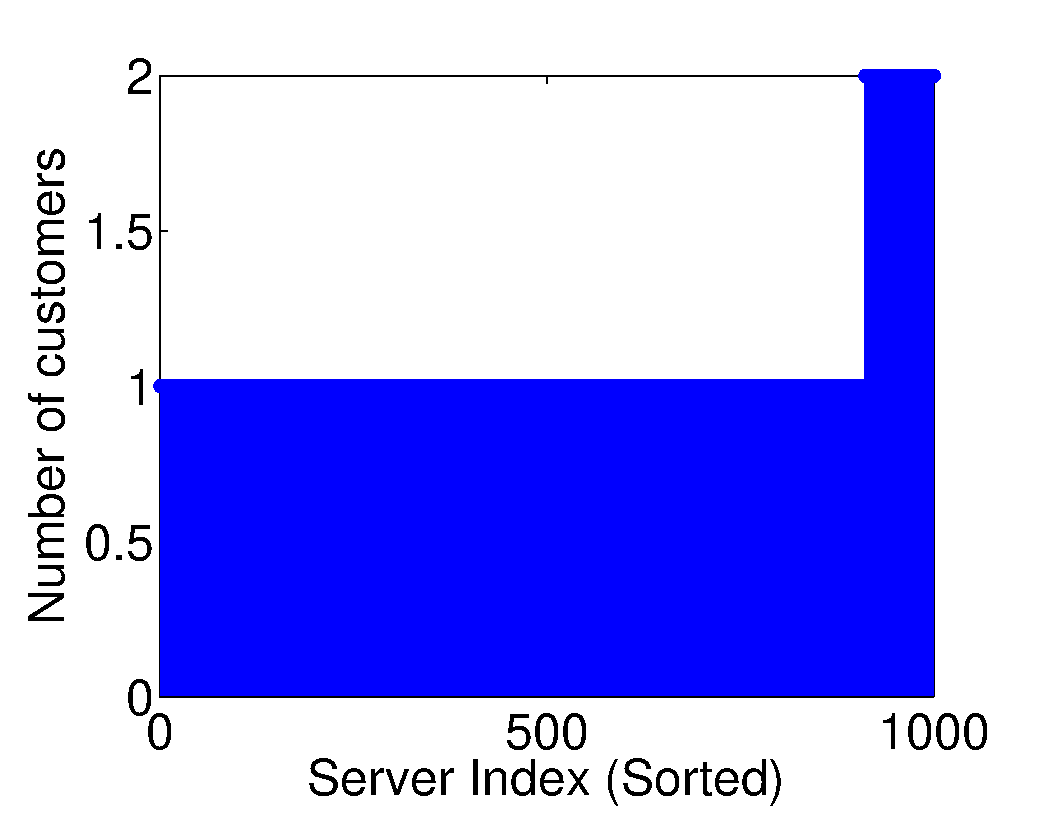
\includegraphics[scale=0.50]{JSQ_quelength.eps}
\caption{Queue length of JSQ with $num of arrivals = 20000$, $n = 1000 \quad servers$, $\lambda = 5000$ and $\mu = 5$.} 
\end{figure}

\begin{figure}[H]
\centering
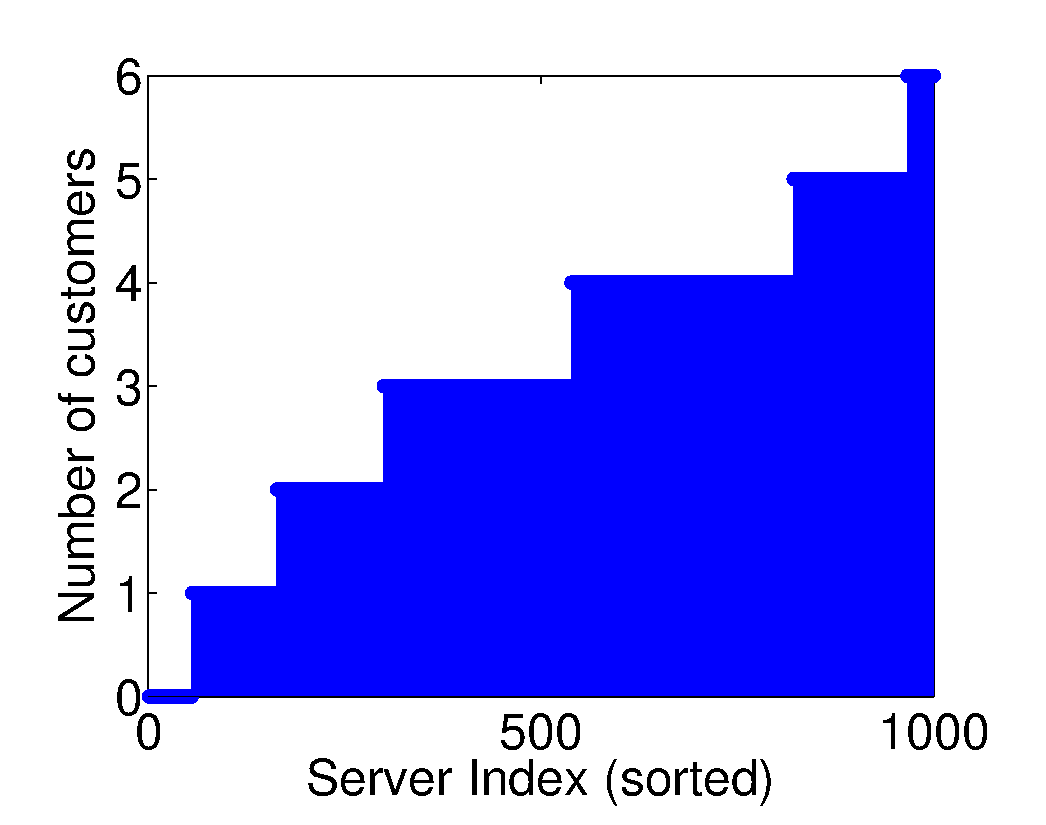
\includegraphics[scale=0.55]{Powerof2_quelengthN1000lambda5000.eps}
\caption{Queue length of ``Power of 2" algorithm with $num of arrivals = 20000$, $n = 1000 \quad servers$, $\lambda = 5000$ and $\mu = 5$.} 
\end{figure}


\begin{figure}[H]
\centering
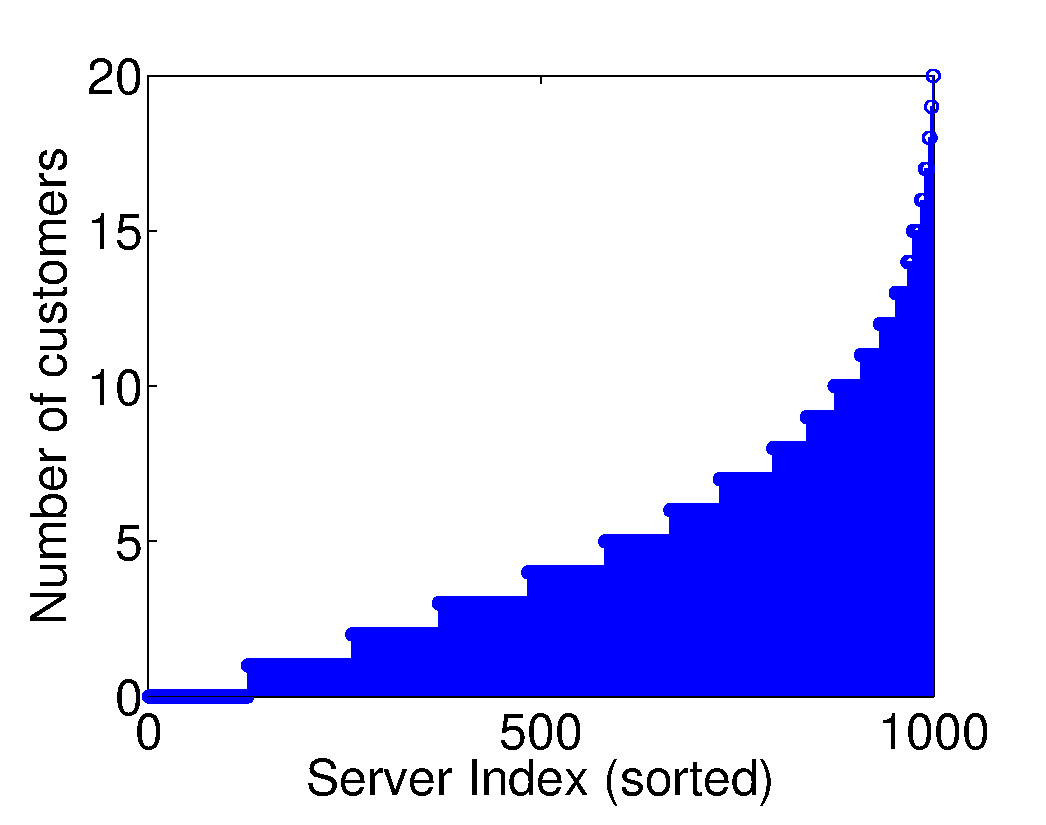
\includegraphics[scale=0.55]{Random_quelength.eps}
\caption{Queue length of purely random strategy with $num of arrivals = 20000$, $n = 1000 \quad servers$, $\lambda = 5000$ and $\mu = 5$.} 
\end{figure}


\begin{figure}[H]
\centering
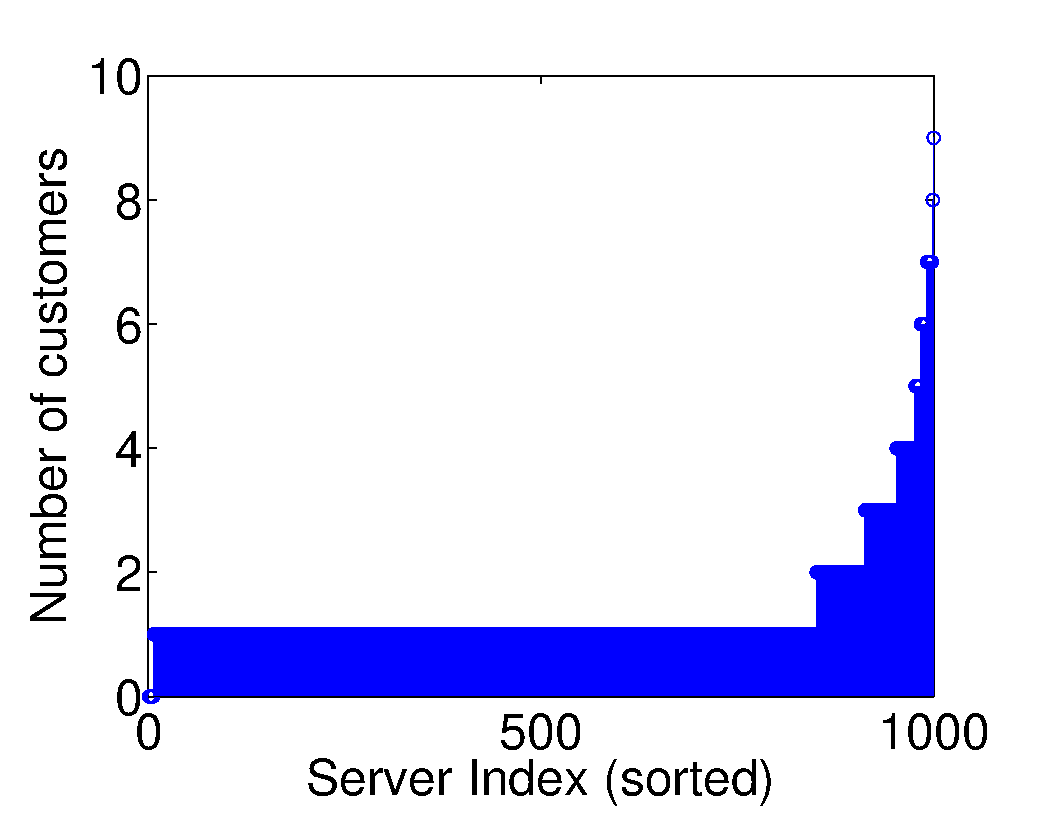
\includegraphics[scale=0.55]{Lastreleiving_quelength.eps}
\caption{Queue length of ``Pick the last relieved" algorithm with $num of arrivals = 20000$, $n = 1000 \quad servers$, $\lambda = 5000$ and $\mu = 5$.} 
\end{figure}

\begin{figure}[H]
\centering
\includegraphics[scale=0.7]{LastreleivingN1000lambda500+Random+JSQ+Powerof2+powerof20+25trials.eps}
\caption{Idle time comparisons of the various algorithms studied with $num of arrivals = 20000$, $n = 1000 \, servers$, $\lambda = 5000$ and $\mu = 5$.} 
\end{figure}
For fig. 1-4, the queue lengths were calculated in the regime when $\lambda = n\mu$.  For clarity of presentation, the queue length of the servers are sorted before they are plotted. For fig. 5, each algorithm was ran for $25$ number of trials and their means and standard deviations are plotted. 
\section{Discussion}
In the previous section we have shown the different plots for the queue lengths and the idle time for the four algorithms for supermarket modeling that we have studied.
\subsection{Discussion of queue lengths}
\par Firstly the work load (as indicated by the queue lengths) of Join the Shortest Queue (JSQ) algorithm as fig. 1 shows turns out to be most efficiently and uniformly distributed among the servers. As long as the system is operating in the stable regime ($\lambda \leq n\mu$) the customers in JSQ are spread uniformly among the servers. This clearly shows the optimality of the JSQ strategy for supermarket modeling.
\par At the other end of the architectural complexity, the purely random stategy as shown in fig. 3 shows a large variance in the distribution of work load among the servers. It seems that the work load is not evenly distributed for this zero-information at the dispatcher strategy. Naturally, since the dispatcher has no information about the queue lengths, it blindly allocates the servers to the incoming arrivals causing some servers to have a huge work load while some servers remain idle.
\par Again, if we allow a subset of $d$ servers to picked uniformly at random and pick the one with minimum queue length then by fig. 2 just by using $d=2$, we can see the far much better distribution of work load among the servers. While here too, we have some servers remaining idle and some having upto 6 customers (as shown in fig. 2 for this case) it performs better than the pure random strategy.
\par Finally, for the ``Pick the last relieved server" algorithm,the queue length distribution results in better performance as compared to the two randomized algorithms as seen in fig. 4. However, still we have a large variance between the maximum and the minimum loaded servers. This strategy can be efficiently utilized in cases when one can afford the limited cost of knowing the last empty server. Clearly, it tends to perform better even than the ``power of 2" startegy which also the additional cost of knowing the queue lengths of the $d$ selected queues.
\subsection{Discussion of idle time}
The idle time as stated before is considered as the time elapsed when a job remains unattended at a server while some other server is empty. This quantity, naturally is a measure of the quality of the algorithm for supermarket model. A lesser idle time for a particular strategy would imply the algorithm is good and vice-versa.
\par The JSQ again in this measure outperforms all other algorithms comprehensively as seen in fig. 5 as here we have the information about the queue lengths of all the servers at each time. Secondly, the ``last relieved server" strategy is also competing very close to the JSQ strategy, again signifying the efficiency for the algorithm. It is natural because the last relieved server would be very likely to get empty before the other servers.
\par For the purely randomized algorithm, the idle time is the highest as was also justified in the previous sub-section. However, the ``power of d" boosts up the performance of the randomized strategy by a significant amount in terms of idle time measurements.

\begin{thebibliography}{11}
\bibitem{Prabhakar}
Bramson, Maury, Yi Lu, and Balaji Prabhakar. ``Asymptotic independence of queues under randomized load balancing." \textit{Queueing Systems} 71.3 (2012): 247-292.
\bibitem{Mitzenmacher}
M. Mitzenmacher, ``The power of two choices in randomized load balancing," Ph.D. dissertation, Univ. Calif, Berkeley, 1996.
\bibitem{Vv}
Vvedenskaya, N.D., Dobrushin, R.L. and Karpelevich, F.I. ``Queueing system
with selection of the shortest of two queues:  An asymptotic approach",Probl  Inf Transm, vol. 32, pp. 20–34, 1996.
\bibitem{Turner}
Turner, S.R.E. ``Resource Pooling in Stochastic Networks", Ph.D. Thesis, Sta-
tistical Laboratory, Christ’s College, University of Cambridge, 1996.
\bibitem{Li}
Quan-Lin Li and Feifei Yang, ``Reward processes and performance simulation in
supermarket models with different servers", in Int. J. of Simulation and Process Modeling, pp. 1-15, 2016.
\bibitem{VvSu} Suhov, Y.M. and Vvedenskaya, N.D. ``Fast Jackson
networks with dynamic routing",
Probl Inf Transm , vol. 38, pp. 136–153, 2002.
\bibitem{Luczak}
 Luczak, M.J. and McDiarmid, C. ``On the maximum queue length in the
supermarket model", The Annals of Probability, vol. 34, pp. 493–527, 2006.
\end{thebibliography}


\end{document}
